\section{Agentic Mechanism}

\subsection{Interleaved Thinking}
\label{sec:interleaved-thinking}

LLM agents must orchestrate multi-step workflows that alternate between natural-language reasoning and external tool invocations such as code execution, web browsing, and API calls. A critical design question is how the model's chain-of-thought (CoT) should interact with tool-use turns, and whether prior reasoning state should be preserved across interaction rounds. In MiniMax-M2, we adopt \textbf{interleaved thinking} as a first-class agent modeling principle: the model alternates between explicit deliberation and tool execution within a single trajectory, carrying the full reasoning state forward across turns.

\noindent \textbf{Interleaved chain-of-thought.} We define interleaved thinking as a generation protocol in which the model produces reasoning tokens $r_t$ and action tokens $a_t$ in an alternating sequence:
\begin{equation}
\tau = (r_1, a_1, o_1, r_2, a_2, o_2, \ldots, r_T, a_T, o_T),
\end{equation}
where $o_t$ denotes the observation (tool output) returned after executing action $a_t$. Each reasoning segment $r_t$ is conditioned on the full history $(r_1, a_1, o_1, \ldots, r_{t-1}, a_{t-1}, o_{t-1})$, allowing the model to revise plans, update hypotheses, and incorporate new evidence before selecting the next action. This contrasts with two common alternatives: (1) front-loaded reasoning, where all reasoning tokens are produced before any actions, preventing adaptation to intermediate observations; and (2) stateless per-turn reasoning, where prior reasoning tokens $r_{<t}$ are stripped from context before generating $r_t$, preventing the model from building on earlier analysis.

\noindent \textbf{Reasoning state persistence.} The key architectural decision enabling interleaved thinking is that the complete model output from turn $t$---including all thinking blocks---is appended to the message history and provided as context for turn $t+1$. Let $\mathcal{H}_t$ denote the conversation history at turn $t$. Under reasoning state persistence:
\begin{equation}
\mathcal{H}_{t+1} = \mathcal{H}_t \oplus [\mathrm{assistant}(r_t, a_t)] \oplus [\mathrm{tool}(o_t)].
\end{equation}
When reasoning state is dropped, history degrades to $\mathcal{H}_{t+1}^{\text{(drop)}} = \mathcal{H}_t \oplus [\mathrm{assistant}(a_t)] \oplus [\mathrm{tool}(o_t)]$, forcing the model to re-derive context, constraints, and partial conclusions at every turn, leading to cumulative state drift and degraded self-correction.

\noindent \textbf{The Plan-Act-Reflect loop.} Interleaved thinking operationalizes a structured cognitive loop at each turn $t$: (1) \textbf{Plan}---the model reviews accumulated state from prior reasoning and observations, then formulates or refines a strategy; (2) \textbf{Act}---the model selects and executes a tool call grounded in the plan; (3) \textbf{Reflect}---the model evaluates the observation against expectations, updates its world model, and determines whether to revise the plan or proceed. This loop enables self-correction through reflection on unexpected observations, sample efficiency by reusing hypotheses and intermediate conclusions rather than re-deriving them, and debuggability via the interpretable reasoning trace. Figure~\ref{fig:interleaved-thinking} illustrates this process.

\begin{figure}[h]
\centering
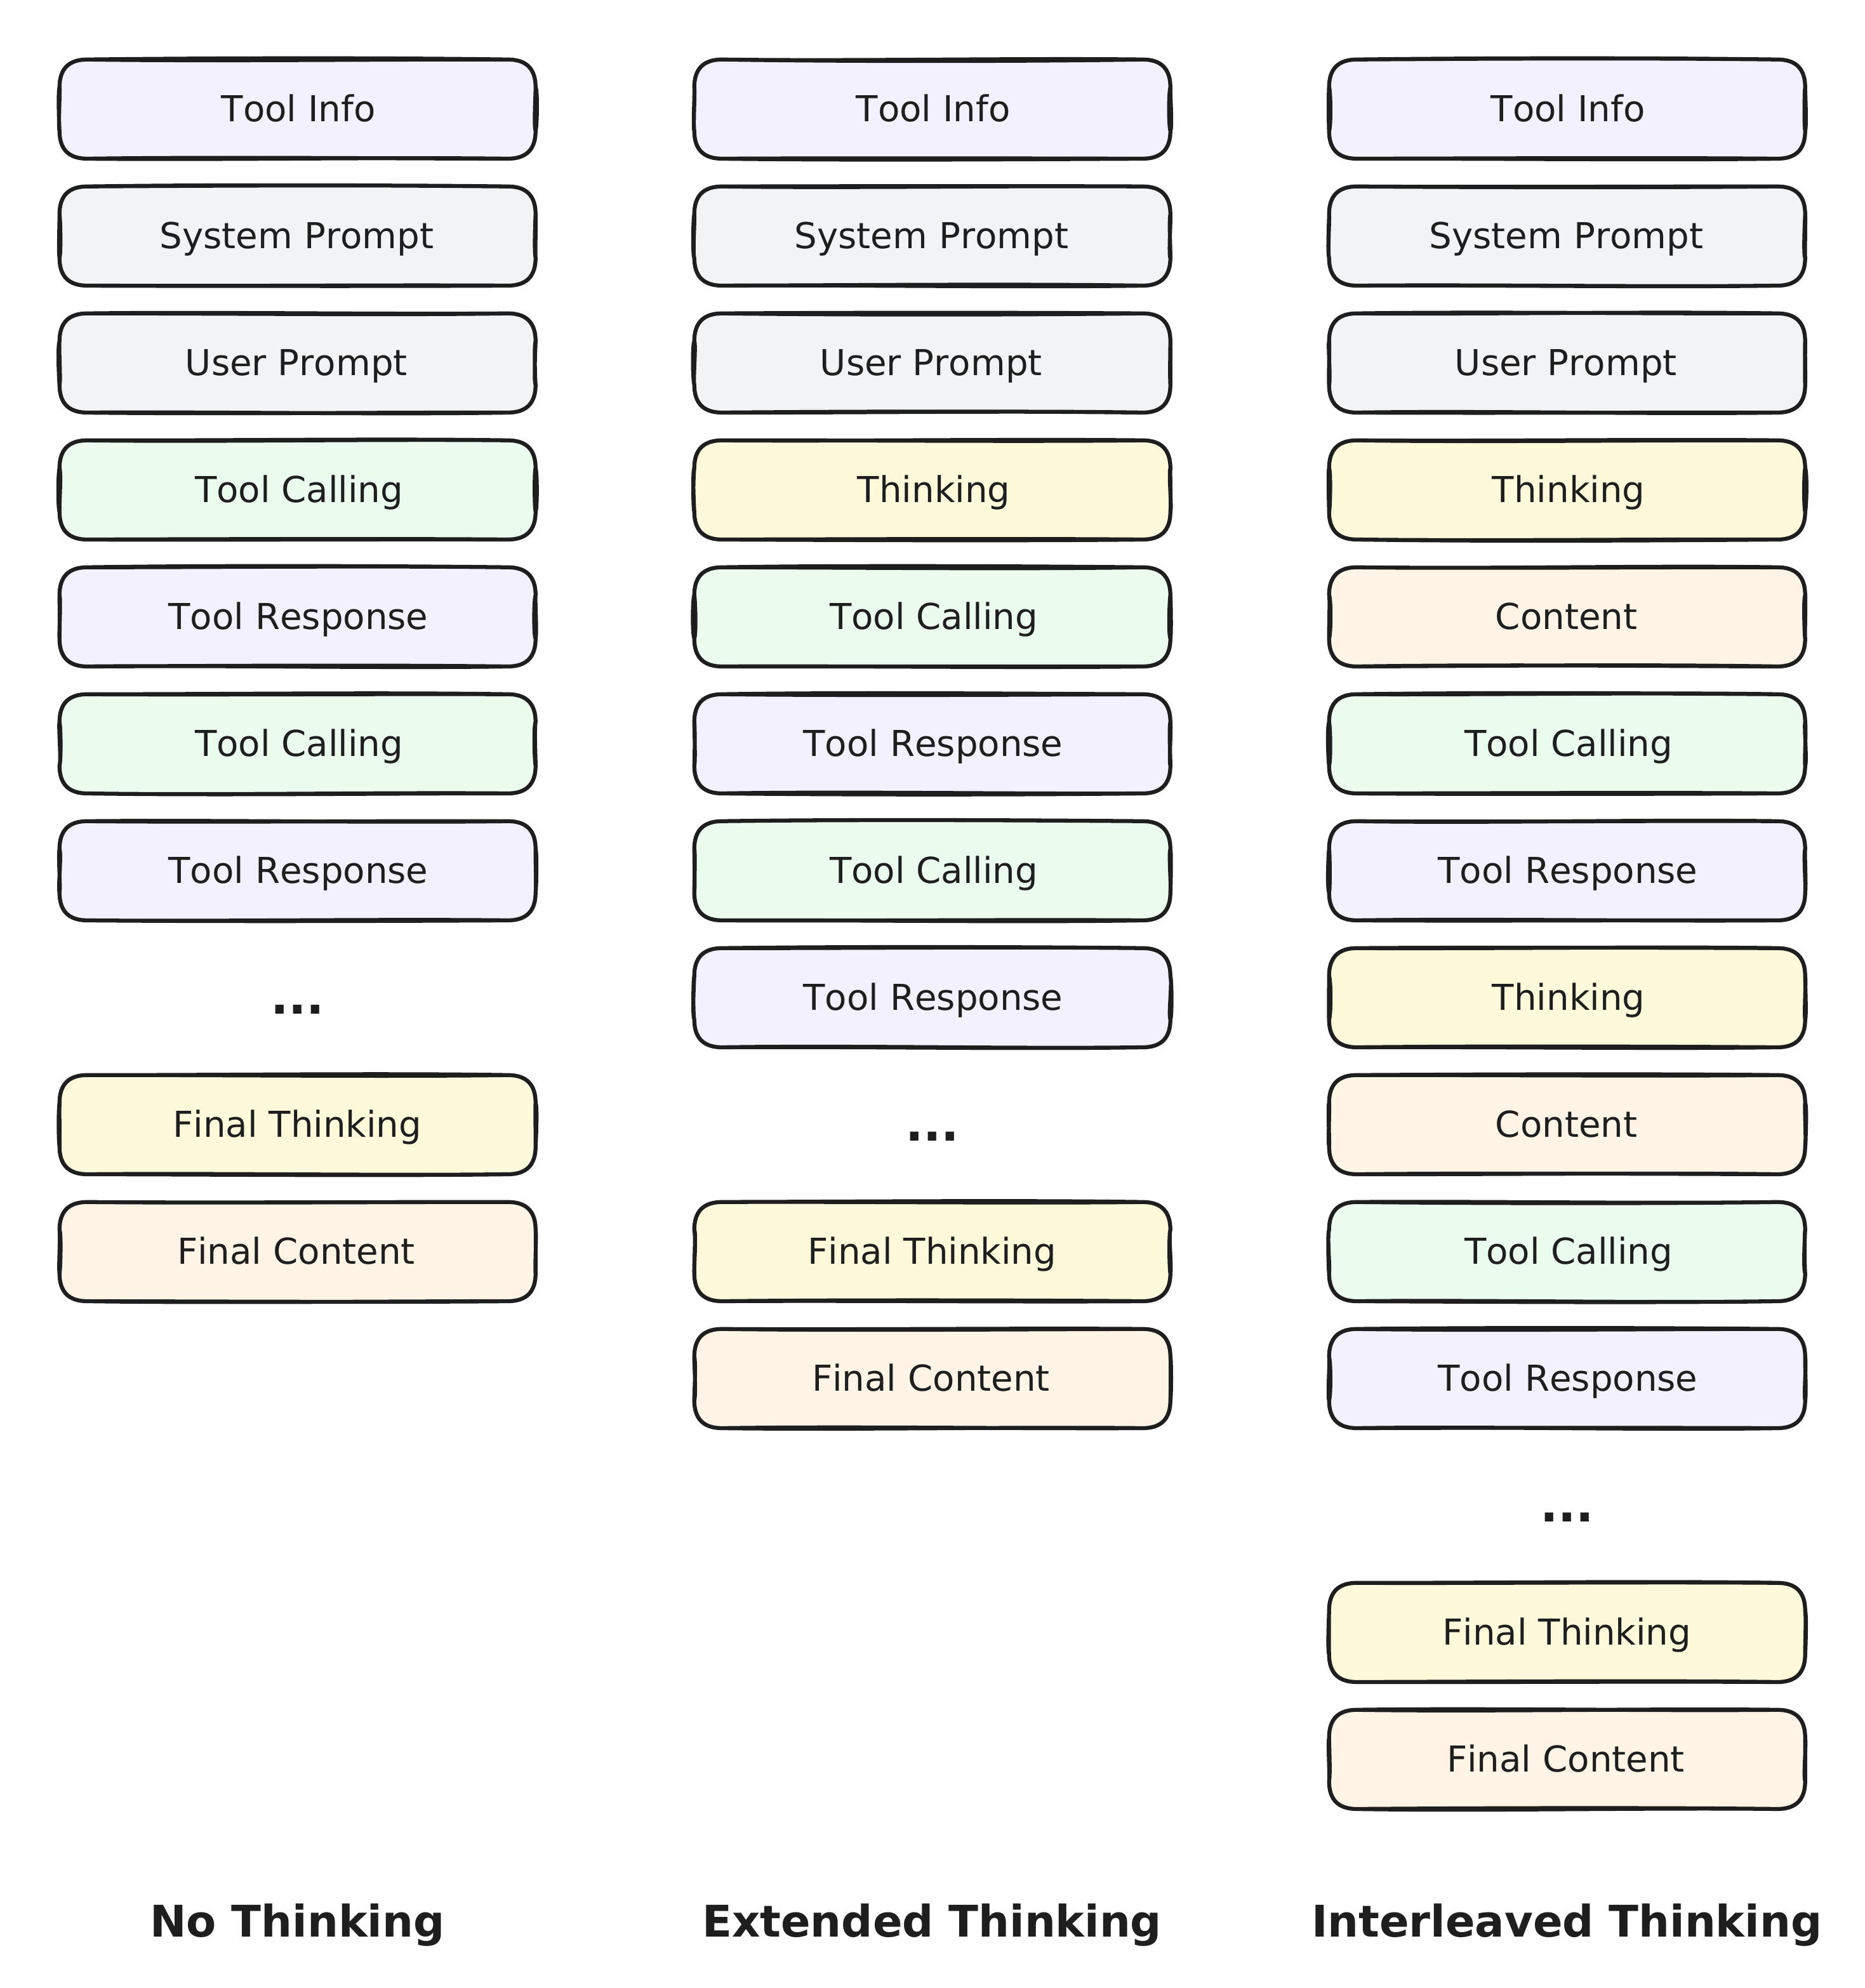
\includegraphics[width=0.65\textwidth]{figures_new/interleaved_thinking.pdf}
\caption{The Plan-Act-Reflect loop of interleaved thinking in M2.}
\label{fig:interleaved-thinking}
\end{figure}

\noindent \textbf{Effect of reasoning state persistence.} We ablate reasoning state persistence by stripping thinking blocks from prior turns before each model invocation, yielding consistent gains across agentic benchmarks, with particularly large improvements on tasks requiring extended multi-step reasoning like deep search and software engineering, indicating that interleaved thinking is most impactful when tasks demand sustained planning and iterative refinement across many steps.

\subsection{Self-Evolution}
\label{sec:self-evolution}

\noindent We detail a shift in model training toward self-evolution. Rather than a sudden leap, this shift represents the culmination of the M2 series' steadily growing agentic capabilities---progressing from routine debugging and reporting tasks into a fully integrated pipeline where M2.7 actively drives its own iterative development (Figure~\ref{fig:self-evolution}).

\noindent To operationalize this, we developed the \textbf{Model Iteration System} (Figure~\ref{fig:self-evolution}A), which operates on the principle that humans steer while models build. Researchers configure goals, guide the agent via chat, and review outputs to decide the next steps. The agent functions within an ``Agent Harness''---a workspace generated entirely by an internal M2.7 model with zero human-written code. This harness equips the model with hierarchical skills for action chaining, persistent memory, safety guardrails, and evaluation infrastructure.

\noindent In practice, our RL team uses this system through a dynamic, dual-loop workflow (Figure~\ref{fig:self-evolution}B). Following human-led experiment planning, M2.7 enters an autonomous execution phase to profile ongoing runs, read logs, and diagnose metric anomalies. By automatically debugging code and adjusting configurations, the model directly intervenes in its training loop, absorbing 30\% to 50\% of the daily iteration workload. Human review triggers major iteration decisions, while the agent can auto-continue bounded analysis between reviews.

\noindent Ultimately, this system enables recursive scaffold upgrades. Tasked with optimizing an internal programming scaffold, M2.7 executed a fully autonomous 100-round iteration cycle: analyzing failures, modifying code, and evaluating changes. This exploration introduced mechanisms such as loop detection and discovered better parameter combinations, yielding a 30\% performance gain on in-house evaluations and showing that the model can improve the infrastructure shaping its subsequent iterations.

\begin{figure}[h]
\centering
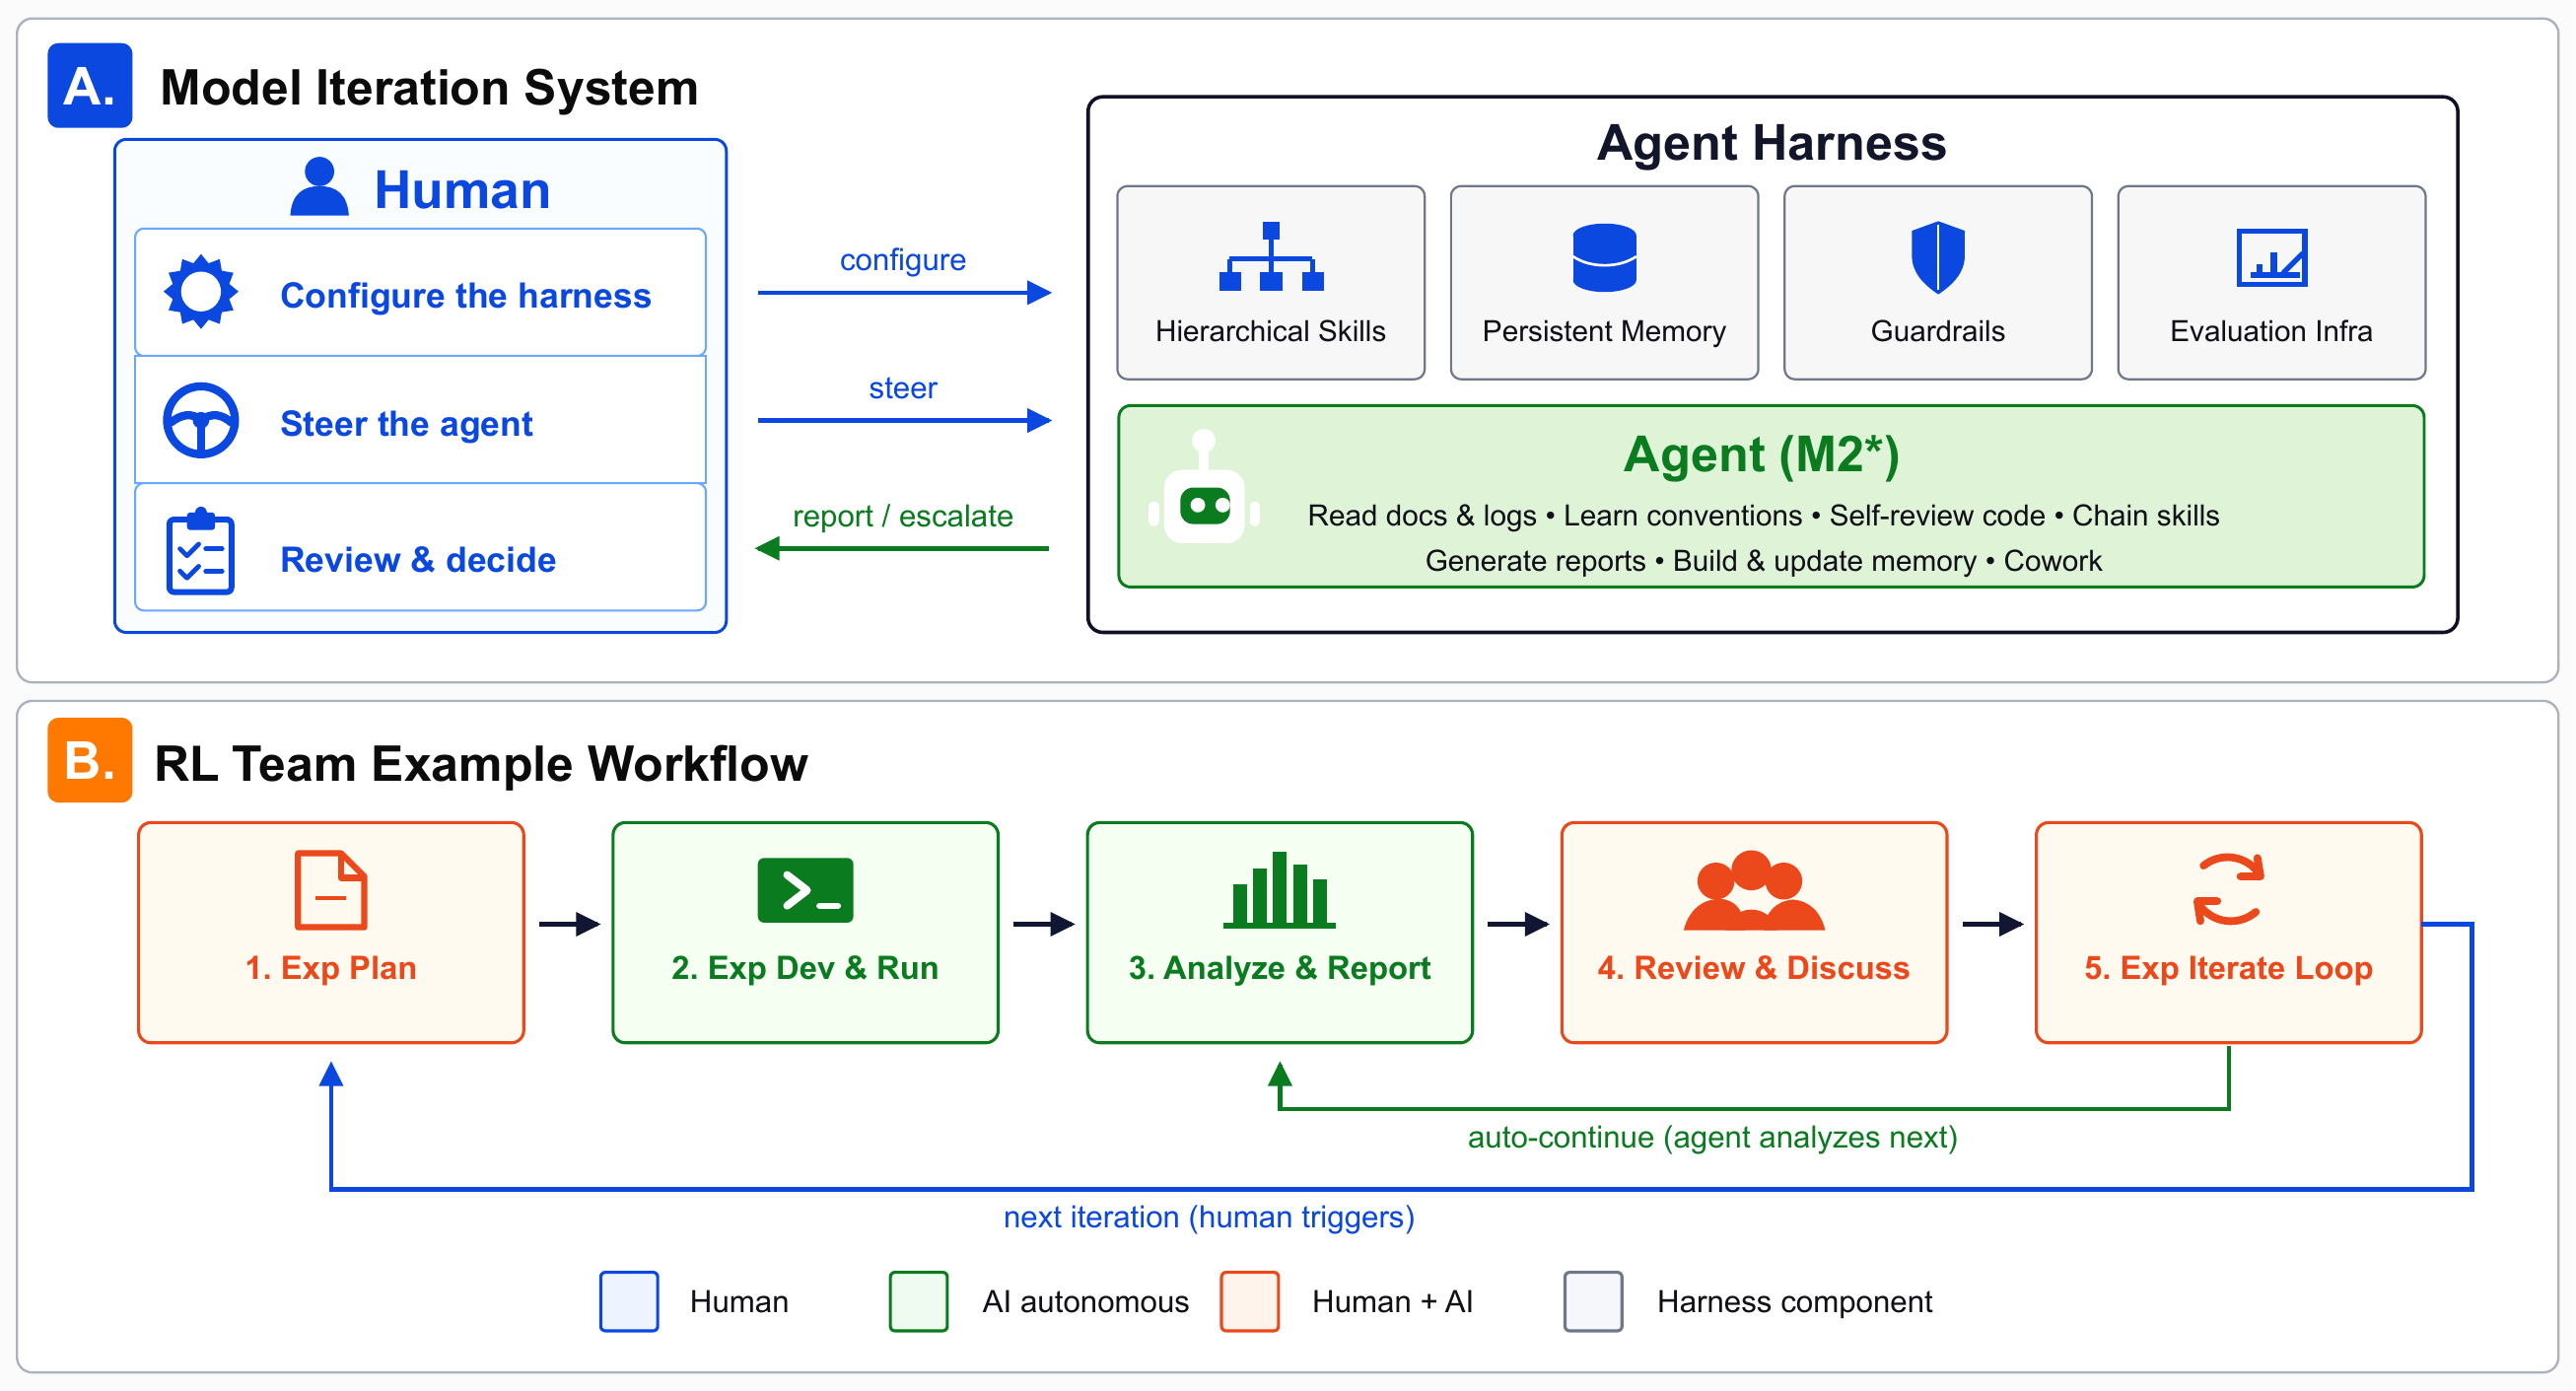
\includegraphics[width=0.9\textwidth]{figures_new/self_evolution.pdf}
\caption{(A) The Model Iteration System used to drive M2.7's autonomous execution. (B) The dual-loop workflow used by our RL team.}
\label{fig:self-evolution}
\end{figure}
